\section{Introduction}

This tutorial demonstrates the usage of {\it BayesX} for
simultaneously selecting variables and smoothing parameters in
semiparametric regression models using {\it stepwisereg objects}. As
an example, we consider data on childhood undernutrition in Zambia.
This data has already been analysed in \citeasnoun{kanlan01} and we
will use the same data set  that has been used there. Since our
focus is on demonstrating how regression models can be estimated in
{\it BayesX}, we do not discuss or interpret the estimation results
but simply give the commands to obtain them.

The main focus in this tutorial is on a method for simultaneously selecting variables and smoothing parameters. {\it BayesX}
also supports two further inferential concepts: full Bayesian inference based on MCMC and empirical Bayes inference based on
mixed model methodology, which are described in two additional tutorials. All tutorials are designed to be self-contained and
describe all features of {\it BayesX} in detail, that will be needed throughout the tutorial. Users who are already familiar
with the usage of {\it dataset} and {\it map objects} may therefore skim through sections \ref{step:usage}--\ref{step:maps}.

The theoretical background of Bayesian semiparametric regression will not be described in this tutorial. The reference manual
may serve as a first introduction, while further details about the estimation techniques employed in this tutorial can be found
in \citeasnoun{bellan08}.

\section{Description of the data set}

Undernutrition among children is usually determined by assessing an anthropometric status of the children relative to a
reference standard. In our example, undernutrition is measured by stunting or insufficient height for age, indicating chronic
undernutrition. Stunting for a child $i$ is determined using a Z-score defined as
\[
Z_i = \frac{AI_i-MAI}{\sigma}
\]
where $AI$ refers to the child`s anthropometric indicator (height at a certain age in our example), while MAI and $\sigma$
correspond to the median and the standard deviation in the reference population, respectively.

Our main interest is in modelling the dependence of undernutrition on covariates including the age of the child, the body mass
index of the child`s mother, the district the child lives in and some further categorial covariates. Table \ref{step:zambiavar}
gives a description of the variables that will be used in our analysis.

{\footnotesize
\begin{table}[ht]
\begin{center}
\begin{tabular}{lp{12.5cm}}
 \hline
 {\bf Variable} & {\bf Description}\\
 \hline
 $\mathit hazstd$ & standardised Z-score for stunting\\
 $\mathit bmi$ & body mass index of the mother\\
 $\mathit agc$ & age of the child in months\\
 $\mathit district$ & district where the mother lives\\
 $\mathit rcw$ & mother`s employment status with categories ``working'' (= 1) and ``not working'' (= $-1$)\\
 $\mathit edu1/2$ & mother`s educational status with categories ``complete primary but incomplete secondary'' ($edu1=1$), ``complete secondary or higher'' ($edu2=1$) and ``no education or incomplete primary'' ($edu1=edu2=-1$)\\
 $\mathit tpr$ & locality of the domicile with categories ``urban'' (= 1) and ``rural'' (= $-1$)\\
 $\mathit sex$ & gender of the child with categories ``male'' (= 1) and  ``female'' (= $-1$)\\
 $\mathit edu$ & mother`s educational status with categories  ``no education or incomplete primary'' ($edu=0$),
 ``complete primary but incomplete secondary'' ($edu=1$) and
 ``complete secondary or higher'' ($edu=2$) \\
 \hline
\end{tabular}
{\it\caption{Variables in the undernutrition data set. \label{step:zambiavar}}}
\end{center}
\end{table}}

\section{Getting started}\label{step:usage}

After having started the graphical user interface version of {\it BayesX}, a main window with four sub-windows appears on the
screen. These are the {\it command window} for entering and executing code, the {\it output window} for displaying results, the
{\it review window} for easy access to past commands, and the {\it object browser} that displays all objects currently
available. In the command line version of {\it BayesX}, there are, of course, no sub-windows but only the command line prompt to
enter commands.

{\it BayesX} is object oriented although the concept is limited, i.e. inheritance and other concepts of object oriented
languages like C++ or R are not supported. For every object type, a number of object-specific methods can be applied to a
particular object instance. The syntax for generating a new object in {\it BayesX} is

{\tt> }{\it objecttype objectname}

where {\it objecttype} defines the type of the object to be created, e.g. {\tt dataset}, and {\it objectname} is the name to be
assigned to the new object.

The rest of the tutorial is separated in seven parts dealing with the different steps of estimating a regression model. In
section \ref{step:datasets}, we create a {\it dataset object} to store, handle and manipulate the data. We will also give a
brief description of some methods that may be applied to {\it dataset objects}. Since we want to estimate a spatial effect of
the district in which a child lives, we need the boundaries of the districts to compute the neighborhood information of the map
of Zambia. This information will be stored in a {\it map object}. \ref{step:maps} describes how to create and handle these
objects. Model selection and estimation of the regression model is carried out in \ref{step:regression} using a {\it
stepwisereg object}. Section \ref{step:confidence} extends the usage of {\it stepwisereg objects} to calculating
credible bands. The next two sections describe how to visualize the estimation results and how to customize the obtained
graphics.

If you have not done so yet, please download the data set and the {\it boundary file} associated with this tutorial now (from
the {\it BayesX} homepage). You may also want to download the batch file containing the commands used in the following
sections. Please note, that paths within these commands must be changed according to the storage location of the corresponding
files on your hard disk.

\section{Reading data set information}\label{step:datasets}

In a first step, we read the available data set information into {\it BayesX}. Therefore we create a {\it dataset object} named
|d|:

|> dataset d|

We store the data in |d| using the method |infile|:

|> d.infile, maxobs=5000 using c:\data\zambia.raw|

Note, that we assume the data to be provided in the external file |c:\data\zambia.raw|. The first few lines of this file look
like this:

{\footnotesize
 hazstd bmi agc district rcw edu1 edu2 tpr sex\\
 0.0791769 \,\, 21.83 \,\, 4 \,\, 81 \,\, -1 \,\, 1 \,\, 0 \,\, 1 \,\, -1\\
 -0.2541965 \,\, 21.83 \,\, 26 \,\, 81 \,\, -1 \,\, 1 \,\, 0 \,\, 1 \,\, -1\\
 -0.1599823 \,\, 20.43 \,\, 56 \,\, 81 \,\, 1 \,\, -1 \,\, -1 \,\, 1 \,\, 1\\
 0.1733911 \,\, 22.27 \,\, 6 \,\, 81 \,\, -1 \,\, 0 \,\, 1 \,\, 1 \,\, 1}

In our example, the file contains the variable names in the first line. It is therefore not necessary to specify the variable names explicitly in the
|infile| command. If the file contained only the data without variable names, we would have to supply them after the keyword
|infile|:

 |> d.infile hazstd bmi agc district rcw edu1 edu2 tpr sex, maxobs=5000|
 |  using c:\data\zambia.raw|

Option |maxobs| can be used to speed up the execution time of the |infile| command. If |maxobs| is specified, {\it BayesX}
allocates enough memory to store all the data while the total amount of required memory is unknown in advance if |maxobs|
remains unspecified. For larger data sets, this may cause {\it BayesX} to start reading the data set information several times
because the currently allocated memory is exceeded. However, this is only meaningful for larger data sets with more than 10,000
observations and could therefore be omitted in our example.

A second option that may be added to the |infile| command is the |missing| option to indicate missing values. Specifying for
example |missing = M| defines the letter `|M|' as an indicator for a missing value. The default for missing values are a period
`.' and `|NA|' (which remain valid indicators for missing values even if an additional indicator is defined by the |missing|
option).

After having read the dataset information, we can inspect the data visually. Executing the command

|> d.describe|

opens an {\it Object-Viewer} window containing the data in form of a spreadsheet (see Figure \ref{step:screenshot}). The same
can also be achieved by double-clicking on the {\it dataset object} in the {\it object browser}.

\vspace{2cm}

\begin{figure}
\begin{center}
\epsfig{file=grafiken/screenshot2.eps,scale=0.5} {\it\caption{A
screenshot of the dataset.\label{step:screenshot}}}
\end{center}
\end{figure}

Further methods allow to examine the variables in the {\it dataset object}. For a categorial variable such as $\mathit{sex}$,
the |tabulate| command may be used to produce a frequency table:

|> d.tabulate sex|

resulting in

\begin{verbatim}
Variable: sex

          Value       Obs           Freq            Cum
             -1      2451         0.5057         0.5057
              1      2396         0.4943              1
\end{verbatim}

being printed in the {\it output window}. For continuous variables,  the |descriptive| command prints several characteristics
of the variable in the {output window}. E.g., executing

|> d.descriptive bmi|

leads to

\begin{verbatim}
   Variable    Obs        Mean      Median         Std         Min         Max
        bmi   4847   21.944349        21.4   3.2879659        12.8       39.29
\end{verbatim}

\section{Map objects}\label{step:maps}

In the following, we will estimate a spatially correlated effect of the district in which a child lives. Therefore we need the
boundaries of the districts in Zambia to compute the neighbourhood information of the map of Zambia. We therefore create a {\it
map object}

|> map m|

and read the boundaries using the |infile| command of {\it map objects}:

|> m.infile using c:\data\zambia.bnd|

Having read the boundary information, {\it BayesX} automatically computes the neighbourhood matrix of the map.

The file following the keyword |using| is assumed to contain the boundaries in form of closed polygons. To give an example we
print a small part of the boundary file of Zambia. The map corresponding to the section of the boundary file can be found in
Figure \ref{step:zambia52}.

\footnotesize

\hspace{1cm}  $\vdots$

 "52",48\\
 28.080507,-12.537530\\
 28.083376,-12.546980\\
 28.109501,-12.548961\\
 28.134972,-12.566787\\
 28.154797,-12.585320\\
 28.165771,-12.593912\\
 28.165771,-12.593912\\
 28.160769,-12.609917\\
 28.152800,-12.633824\\
 28.144831,-12.657733\\
 28.132877,-12.677656\\
 28.120922,-12.701565\\
 28.120922,-12.717505\\
 28.120922,-12.741411\\
 28.116938,-12.761335\\
 28.108969,-12.777274\\
 28.100998,-12.793213\\
 28.089045,-12.817122\\
 28.085060,-12.837045\\
 28.081076,-12.856968\\
 28.081076,-12.876892\\
 28.080862,-12.884153\\
 28.080862,-12.884153\\
 28.076630,-12.879521\\
 28.031454,-12.881046\\
 27.974281,-12.884675\\
 27.910725,-12.878692\\
 27.686228,-12.880120\\
 27.665676,-12.854732\\
 27.653563,-12.818301\\
 27.639263,-12.759848\\
 27.648254,-12.699927\\
 27.662464,-12.680613\\
 27.662464,-12.680613\\
 27.666534,-12.675080\\
 27.703260,-12.679779\\
 27.752020,-12.695455\\
 27.797932,-12.702188\\
 27.836775,-12.707567\\
 27.867813,-12.699892\\
 27.902308,-12.667418\\
 27.922668,-12.630853\\
 27.943035,-12.596350\\
 27.963434,-12.571486\\
 27.983179,-12.563844\\
 28.016331,-12.554779\\
 28.070650,-12.542199\\
 28.080507,-12.537530\\

\hspace{1cm} $\vdots$

\normalsize

\vspace{0.3cm}

For each region of the map, the boundary file must contain the identifying name of the region, the polygons that form the
boundary of the region, and the number of lines the polygon consists of. The first line always contains the region code
surrounded by quotation marks and the number of lines the polygon of the region consists of. The code and the number of lines
must be separated by a comma. The subsequent lines contain the coordinates of the straight lines that form the boundary of the
region. The straight lines are represented by the coordinates of their end points. Coordinates must be separated by a comma.
Note that the first and the last point must be identical (see the example above) to obtain a closed polygon. Compare chapter 5
of the reference manual for a detailed description of some special cases, e.g. regions divided into subregions.

\begin{figure}[h]
\centering

\includegraphics [scale=0.3]{grafiken/zambia52.ps}
\caption{\label{step:zambia52} Corresponding graph of the section of
the boundary file}
\end{figure}

{\it Map objects} may be visualised using method |describe|:

|> m.describe|

resulting in the graph shown in Figure \ref{step:zambiamap}. Additionally, |describe| prints further information about the {\it
map object} in the {\it output window} including the name of the object, the number of regions, the minimum and maximum number
of neighbours and the bandwidth of the corresponding adjacency or neighbourhood matrix:

\begin{verbatim}
  MAP m
  Number of regions: 54
  Minimum number of neighbors: 1
  Maximum number of neighbors: 9
  Bandsize of corresponding adjacency matrix: 24
\end{verbatim}

\begin{figure}[ht]
\begin{center}
\epsfig{file=grafiken/zambia.ps,scale=0.35} {\it\caption{The
districts within Zambia.\label{step:zambiamap}}}
\end{center}
\end{figure}


The numerical complexity associated with the estimation of structured spatial effects depends essentially on the structure of
the neighbourhood matrix. Often the geographical information stored in a boundary file does not represent the ``ideal''
ordering of the districts or regions (with respect to the estimation problem). Therefore it may be useful to reorder the map
using method |reorder|:

|> m.reorder|

Usually, reordering results in a smaller bandwidth although the bandwidth is not the criterion that is minimised by |reorder|.
Instead the {\it envelope} of the neighbourhood matrix is minimised (compare \citeasnoun{geoliu81}).

In order to avoid reordering the {\it map object} every time you start {\it BayesX}, it is useful to store the reordered
version in a separate file. This can be achieved using the |outfile| command of {\it map objects}:

|> m.outfile, replace using c:\data\zambiasort.bnd|

The reordered map is now stored in the given file. Note, that specifying the option |replace| allows {\it BayesX} to overwrite
an existing file with the same name. Without this option, an error message would be raised if the given file is already
existing.

Reading the boundary information from an external file and computing the neighbourhood matrix may be a computationally
intensive task if the map contains a large number of regions or if the polygons are given in great detail. To avoid doing these
computation in every {\it BayesX} session, we store the neighbourhood information in a {\it graph file} using method |outfile|
together with the |graph| option:

|> m.outfile, replace graph using c:\data\zambiasort.gra|

A graph file stores the nodes and the edges of a graph $G = (N,E)$, see for example \citeasnoun{geoliu81} for a first
introduction into graph theory. A graph is a convenient way of representing the neighbourhood structure of a geographical map.
The nodes of the graph correspond to the region codes. The neighbourhood structure is represented by the edges of the graph. In
some situations it may be useful to define weights associated with the edges of a graph which can be be stored in the {\it
graph file} as well.

We now describe the structure of a graph file as it is expected by {\it BayesX}. The first line of a {\it graph file} must
contain the total number of nodes of the graph. In the remaining lines, the nodes of the graph together with their edges and
associated weights are specified. One node corresponds to three consecutive lines. The first of the three lines must contain
the name of the node, which typically will be the name of the geographical region. In the second line, the number of edges of
that particular node is given. The third line contains the corresponding edges of the node, where an edge is given by the index
of a neighbouring node. The index starts with zero. For example, if the fourth and the seventh node/region in the {\it graph
file} are connected/neighbours, the edge index for the fourth node/region is 6 and for the seventh node/region 3.

We illustrate the structure of a graph file with an example. The following few lines are the beginning of the graph file
corresponding to the reordered map of Zambia:

\footnotesize

 57\\
 87\\
 1\\
 5\\
 76\\
 3\\
 9 8 7\\
 67\\
 2\\
 10 9\\

\hspace{1cm} $\vdots$

\normalsize

\vspace{0.5cm}

The first line specifies the total number of nodes, in the present example 57 nodes. The subsequent three lines correspond to
the node with name `87', which is the first region in the reordered map of Zambia. Region `87' has 1 neighbour, namely the
sixth node appearing in the graph file. Once again, note that the index starts with zero, i.e. 0 corresponds to the first node,
1 corresponds to the second node and so on. Lines 5 to 7 in the example correspond to node `76' and its three neighbours and
lines 8 to 10 correspond to node `67'.

In a graph file it is also possible to specify weights associated with the edges of the nodes. Since in the preceding example
no weights are explicitly specified, all weights are automatically defined to be equal to one. Nonequal weights are specified
in the graph file by simply adding them following the edges of a particular node. An example of the beginning of a graph file
with weights is given below:

\footnotesize

 57\\
 87\\
 1\\
 5 1.44172\\
 76\\
 3\\
 7 8 9 0.707424 1.3816 0.682372\\
 67\\
 2\\
 9 10 1.67424 0.8406\\

\hspace{1cm} $\vdots$

\normalsize

\vspace{0.5cm}

Here the edge of the first node `87' has weight 1.44172, the edges of the second node have weights 0.707424, 1.3816 and
0.682372.

Note, that graph files allow the estimation of very general correlated effects based on Markov random fields. While the
polygons stored in a {\it boundary file} represent geographical information, the nodes and edges of a graph may define
arbitrary neighbourhood structures. For example, the definition of three-dimensional Markov random fields representing
space-time interactions is possible.

To see how storing maps in {\it graph files} affects the computation time of the |infile| command, we create a second {\it map
object} and read in the information from the graph file. Again, we have to specify the keyword |graph|:

\begin{verbatim}
> map m1
> m1.infile, graph using c:\data\zambiasort.gra
\end{verbatim}

As you should have noticed, reading geographical information from a {\it graph file} is usually much faster than reading from a
{\it boundary file}. However, using {\it graph files} also has a drawback. Since they do no longer contain the full information
on the polygons forming the map, we can not visualise a {\it map object} created from a {\it graph file}. Trying to do so

|> m1.describe|

raises an error message. This implies, that visualising estimation results of spatial effects can only be based on {\it map
objects} created from {\it boundary files}, although estimation can be carried out using {\it graph files}. Since we will work
with the {\it map object} |m| in the following, we delete |m1|:

|> drop m1|

\section[Simultaneously selecting variables and smoothing parameters]{Simultaneous selection of variables and smoothing parameters}
\label{step:regression}

To perform  simultaneous selection of variables and smoothing parameters in regression models, we first create a {\it
stepwisereg object}:

|> stepwisereg s|

By default, estimation results are written to the subdirectory |output| of the installation directory. In this case, the
default filenames are composed of the name of the {\it stepwisereg object} and the type of the specific file. Usually it is
more convenient to store the results in a user-specified directory. To define this directory we use the |outfile| command of
{\it stepwisereg objects}:

|> s.outfile = c:\data\s|

Note, that |outfile| does not only specify a directory but also a base filename (the character `s' in our example). Therefore
executing the command above leads to storage of the results in the directory |c:\data| and all filenames start with the
character `s'. Of course the base filename may be different from the name of the {\it stepwisereg object}.

In addition to parameter estimates of the selected model, {\it BayesX} also gives some further information on the selection
process. Not all of this information is stored automatically but is printed in the {\it output window}. Therefore it is useful
to store the contents of the {\it output window}. This is achieved by opening a log file using the |logopen|
command

|> logopen, replace using c:\data\logstep.txt|

After opening a log file, every information written to the {\it output window} is also stored in the log file. Option |replace|
allows {\it BayesX} to overwrite an existing file with the same name as the specified log file. Without |replace| results are
appended to an existing file.

The model presented in Kandala et al.~(2001) is given by the following semiparametric predictor:
\[\eta=\gamma_0+\gamma_1rcw+\gamma_2edu1+\gamma_3edu2+\gamma_4tpr+\gamma_5sex+f_1(bmi)+f_2(agc)+f^{str}(district)+f^{unstr}(district)\]
The two continuous covariates |bmi| and |agc| are assumed to have a possibly nonlinear effect on the Z-score and, therefore,
are modeled nonparametrically (using P-splines with second order difference penalty in our example). However, a linear effect
could be more appropriate and, hence, the linear effect is also considered for model selection. The spatial effect of the
district is split up into a spatially correlated part $f^{str}(district)$ and an uncorrelated part $f^{unstr}(district)$, see
Fahrmeir and Lang (2001b) for a motivation. The correlated part is modeled by a (quadratic) pairwise difference penalty, where the
neighborhood matrix and possible weights associated with the neighbors are obtained from the {\it map object} |m|. The
uncorrelated part is modelled by an i.i.d.~Gaussian random effect (simple ridge type penalty). For each variable and function,
the selection procedure additionally considers the possibility of removing the term from the model.
Both effect variables |edu1| and |edu2| represent
the overall effect of the categorical variable |edu|.  Therefore the variable
|edu| is specified as a {\tt factor} for the selection procedure.


To estimate the model we use method |regress| of {\it stepwisereg objects}:

 |> s.regress hazstd = rcw + edu(factor) + tpr + sex + bmi(psplinerw2)|\\
 |  + agc(psplinerw2) + district(spatial,map=m) + district(random),|\\
 |  family=gaussian predict using d|

%Option {\tt startmodel} ???????????????

If option {\tt predict} is specified estimates for the linear predictor and the expectation of every observation are obtained.

In the following we reproduce the content of the {\it output window} to make the user familiar with the estimation results
produced by {\it BayesX}:

\footnotesize
\begin{verbatim}
STEPWISE PROCEDURE STARTED


  Startmodel:

  hazstd = const
  AIC_imp = 1.0027031

  Startmodel:

  hazstd = const + tpr + sex + edu_1 + edu_2 + bmi +
           agc(psplinerw2,df=10.959,(lambda=15.4071)) +
           district(spatial,df=29.5919,(lambda=7.5775)) +
           district(random,df=9.84981,(lambda=83.6814))
  AIC_imp = -1016.8085

  Startmodel:

  hazstd = const + tpr + sex + edu_1 + edu_2 + bmi +
           agc(psplinerw2,df=10.959,(lambda=15.4071)) +
           district(spatial,df=29.1827,(lambda=6.10614)) +
           district(random,df=12.817,(lambda=50.9029))
  AIC_imp = -1020.7741

  Startmodel:

  hazstd = const + tpr + sex + edu_1 + edu_2 + bmi +
           agc(psplinerw2,df=10.959,(lambda=15.4071)) +
           district(spatial,df=28.0688,(lambda=6.10614)) +
           district(random,df=14.4345,(lambda=42.9308))
  AIC_imp = -1022.474

  Startmodel:

  hazstd = const + tpr + sex + edu_1 + edu_2 + bmi +
           agc(psplinerw2,df=10.959,(lambda=15.4071)) +
           district(spatial,df=28.0688,(lambda=6.10614)) +
           district(random,df=14.4345,(lambda=42.9308))
  AIC_imp = -1023.2235

  Startmodel:

  hazstd = const + tpr + sex + edu_1 + edu_2 + bmi +
           agc(psplinerw2,df=10.959,(lambda=15.4071)) +
           district(spatial,df=25.6558,(lambda=7.5775)) +
           district(random,df=15.8985,(lambda=42.9308))
  AIC_imp = -1024.7078

  Startmodel:

  hazstd = const + tpr + sex + edu_1 + edu_2 + bmi +
          agc(psplinerw2,df=10.959,(lambda=15.4071)) +
          district(spatial,df=25.6558,(lambda=7.5775)) +
          district(random,df=15.8985,(lambda=42.9308))
  AIC_imp = -1024.7018

  Startmodel:

  hazstd = const + tpr + sex + edu_1 + edu_2 + bmi +
           agc(psplinerw2,df=10.959,(lambda=15.4071)) +
           district(spatial,df=24.3664,(lambda=7.5775)) +
           district(random,df=17.8721,(lambda=35.6851))
  AIC_imp = -1024.7455

  Startmodel:

  hazstd = const + tpr + sex + edu_1 + edu_2 + bmi +
           agc(psplinerw2,df=10.959,(lambda=15.4071)) +
           district(spatial,df=24.3664,(lambda=7.5775)) +
           district(random,df=17.8721,(lambda=35.6851))
  AIC_imp = -1024.4848

  Startmodel:

  hazstd = const + tpr + sex + edu_1 + edu_2 + bmi +
           agc(psplinerw2,df=10.959,(lambda=15.4071)) +
           district(spatial,df=24.3664,(lambda=7.5775)) +
           district(random,df=17.8721,(lambda=35.6851))
  AIC_imp = -1024.4091

  Final Model:

  hazstd = const + tpr + sex + edu_1 + edu_2 + bmi +
           agc(psplinerw2,df=10.959,(lambda=15.4071)) +
           district(spatial,df=24.3664,(lambda=7.5775)) +
           district(random,df=17.8721,(lambda=35.6851))
  AIC_imp = -1024.3814

  Used number of iterations: 10

  ------------------------------------------------------------------------
  ------------------------------------------------------------------------

  Final Model:

  hazstd = const + tpr + sex + edu_1 + edu_2 + bmi +
           agc(psplinerw2,df=10.959,(lambda=15.4071)) +
           district(spatial,df=24.3664,(lambda=7.5775)) +
           district(random,df=17.8721,(lambda=35.6851))
  AIC_imp = -1024.352


RESPONSE DISTRIBUTION:

  Gaussian
  Number of observations: 4847


ESTIMATION RESULTS:


  Predicted values:

  Estimated mean of predictors, expectation of response and
  individual deviances are stored in file
  c:\bayesx\output\s_predictmean.raw


  Saturated deviance: 4847

  Estimation results for the scale parameter:

  sigma2:         0.789725



  FixedEffects1

  Variable  mean           Std. Dev.      2.5% quant.    median         97.5% quant.
  const     -0.422865      0              0              0              0
  tpr       0.0945051      0              0              0              0
  sex       -0.0589084     0              0              0              0
  edu_1     -0.063032      0              0              0              0
  edu_2     0.234741       0              0              0              0
  bmi       0.0209163      0              0              0              0

  Results for fixed effects are also stored in file
  c:\bayesx\output\s_FixedEffects1.res


  f_agc

  Results are stored in file
  c:\bayesx\output\s_f_agc_pspline.res

  Results may be visualized using the R / S-Plus function 'plotnonp'
  Type for example:
  plotnonp("c:\\bayesx\\output\\s_f_agc_pspline.res")


  f_district

  Results are stored in file
  c:\bayesx\output\s_f_district_spatial.res

  Results may be visualized using the R / S-Plus function
 'drawmap'


  f_district

  Results for random effects are stored in file
  c:\bayesx\output\s_f_district_random.res

  Results for the sum of the structured and unstructured
  spatial effects are stored in file
  c:\bayesx\output\s_district_spatialtotal.res

  Files of model summary:

  ---------------------------------------------------------------------------

  Batch file for visualizing effects of nonlinear functions is stored in file
  c:\bayesx\output\s_graphics.prg

  NOTE: 'input filename' must be substituted by the filename of the boundary-file

  ---------------------------------------------------------------------------

  Batch file for visualizing effects of nonlinear functions
  in S-Plus is stored in file
  c:\bayesx\output\s_splus.txt

  NOTE: 'input filename' must be substituted by the filename of the boundary-file

  ---------------------------------------------------------------------------

  Latex file of model summary is stored in file
  c:\bayesx\output\s_model_summary.tex

  ---------------------------------------------------------------------------
\end{verbatim}
\normalsize

Note that variable {\it rcw} was removed from the model and variable {\it bmi} is modelled by a linear effect.

In addition to the information being printed to the {\it output window} results for each effect are written to external ASCII
files. The names of these files are given in the {\it output window}, compare the previous pages. The files contain the
posterior mean. For example, the beginning of file |c:\data\s_f_age_pspline.res| for the effect of |age| looks like this:

{\footnotesize
intnr \,\, age \,\, pmean \,\, pqu2p5 \,\, pqu10 \,\, pmed \,\, pqu90 \,\, pqu97p5 \,\, pcat95 \,\, pcat80\\
1 \,\,  0 \,\,  1.0981 \,\,  0 \,\,  0 \,\,  0 \,\,  0 \,\,  0 \,\,  0 \,\,  0 \\
2 \,\,  1 \,\,  0.978917 \,\,  0 \,\,  0 \,\,  0 \,\,  0 \,\,  0 \,\,  0 \,\,  0 \\
3 \,\,  2 \,\,  0.867664 \,\,  0  \,\, 0 \,\,  0 \,\,  0 \,\,  0 \,\,  0 \,\,  0}

Note, that columns {\it pmean} to {\it pcat80} contain no values. Methods for obtaining values for median, posterior 2.5\%,
10\%, 90\% and 97.5\% quantiles, and corresponding 95\% and 80\% posterior probabilities of the estimated effects are described
in section \ref{step:confidence}.

Some nonparametric effects are visualized by {\it BayesX} automatically and the resulting graphs are stored in ps format.
E.g.~the effect of |age| is visualized in the file |c:\data\s_f_age_pspline.ps| (compare the results on the previous pages for
the other filenames). In addition to the postscript files a file containing the commands to reproduce the graphics is stored in
the output directory. In our example the name of the file is |c:\data\s_graphics.prg|. The advantage is that additional options
may be added by the user to customize the graphs (compare the respective two subsubsections).

Moreover a file with ending |.tex| is created in the outfile directory. This file contains a summary of the estimation results
and may be compiled using \LaTeX.

There are two results files containing information about the selection process. File |c:\data\s_models.raw| contains the base
models used at the beginning of each iteration and the finally selected model. File |c:\data\s_criterium.raw| shows changes in
the value of the selection criterion during the selection process.

Having finished the estimation we may close the log file by typing

|> logclose|

Note, that the log file is closed automatically when you exit {\it BayesX}.


\section{Selection including calculation of confidence bands}\label{step:confidence}

{\it stepwisereg objects} allow both the calculation of conditional and unconditional confidence bands for nonlinear functions.

\subsection{Conditional confidence bands}\label{step:cond}

Conditional confidence bands are calculated conditional on the selected model, i.e.~they are computed for selected variables
and functions only. The computation of conditional confidence bands is based on an  MCMC-algorithm subsequent to the
selection procedure. For the selection of a model with an adjacent computation of conditional confidence bands we can use
method |regress| of {\it stepwisereg objects}:

 |> s.regress hazstd = rcw + edu(factor) + tpr + sex + bmi(psplinerw2)|\\
 |  + agc(psplinerw2) + district(spatial,map=m) + district(random),|\\
 |  CI=MCMCselect step=10 iterations=10000 |\\
 |  family=gaussian predict using d|

Options {\tt iterations} and {\tt step} define properties of the MCMC-algorithm. The total number of MCMC iterations is given
by {\tt iterations}. Since, in general, these random numbers are correlated, we do not use all of them but thin out the Markov
chain by the thinning parameter {\tt step}. Specifying {\tt step=10} as above forces {\it BayesX} to store only every 10th
sampled parameter which leads to a random sample of length 1000 for every parameter in our example.

Note, that the choice of {\tt iterations} also affects computation time. On a 2.4 GHz PC estimation of our model took about ?
minute and ? seconds, which is rather fast in regard of the complexity of the model.

Now, file |c:\data\s_f_age_pspline.res| for the effect of |age| contains also results for median, posterior 2.5\%, 10\%, 90\%
and 97.5\% quantiles, and corresponding 95\% and 80\% posterior probabilities of the estimated effects. The first few lines  of the
file looks like this:

{\footnotesize
 intnr \,\, age \,\, pmean \,\, pqu2p5 \,\, pqu10 \,\, pmed \,\, pqu90 \,\, pqu97p5 \,\, pcat95 \,\, pcat80\\
1 \,\,  0 \,\,  1.09481 \,\,  0.925783 \,\,  0.984814  \,\, 1.09623  \,\, 1.20131  \,\, 1.26294 \,\,  1 \,\,  1 \\
2 \,\,  1 \,\,  0.977488 \,\,  0.866704 \,\,  0.906176 \,\,  0.977659  \,\, 1.04638  \,\, 1.08583 \,\,  1 \,\,  1 \\
3 \,\,  2 \,\,  0.867545 \,\,  0.787211 \,\,  0.815846 \,\,  0.8677 \,\,  0.918947 \,\,  0.945463 \,\,  1 \,\,  1}

The posterior quantiles and posterior probabilities may be changed by the user using the options |level1| and |level2|. For
example specifying |level1=99| and |level2=70| in the options list of the |regress| command leads to the computation of 0.5\%,
15\%, 85\% and 99.5\% quantiles of the posterior. The defaults are |level1=95| and |level2=80|.


\subsection{Unconditional confidence bands}\label{step:uncond}

Unconditional confidence bands consider the uncertainty due to model selection. Unconditional confidence bands are obtained using the following modified
 |regress| command:

 |> s.regress hazstd = rcw + edu(factor) + tpr + sex + bmi(psplinerw2)|\\
 |  + agc(psplinerw2) + district(spatial,map=m) + district(random),|\\
 |  CI=MCMCbootstrap bootstrapsamples=99 step=10 iterations=10000 |\\
 |  family=gaussian predict using d|

Options {\tt iterations} and {\tt step} define properties of the MCMC-algorithm. The number of {\tt iterations} is
divided equally between the bootstrap iterations. Here, for each of the 99 bootstrap data sets (specified by {\it
bootstrapsamples=99}) and the original data set 100 MCMC samples are drawn. The thinning parameter is {\tt step =10}, i.e. every  10th
sampled parameter per data set (i.e.~1000 samples altogether) are used for the computation of empirical quantiles. Note, that the number
of bootstrap data sets strongly affects computation time.

In addition to confidence bands, a kind of sensitivity analysis regarding model selection can be performed using the estimation
results. For the effect of |age|, file |c:\data\s_f_age_pspline_df.raw| contains the number of times each modelling alternative
was selected during the bootstrapping process. This frequency distribution indicates the plausibility of the different
modelling alternatives, especially of the modelling alternative selected for the original data. The first few lines of file
|c:\data\s_f_age_pspline_df.raw| looks like this:

{\footnotesize
df\_value \,\,   sp\_value \,\, frequency \,\, selected \\
3.95883 \,\,  1767.34  \,\, 1  \,\, - \\
5.0261 \,\,  634.521 \,\,  21  \,\, - \\
5.96806 \,\,  297.13 \,\,  12 \,\,  -}


\section{Visualizing estimation results}\label{step:visual}

{\it BayesX} provides three alternatives  for visualizing estimation results:
\begin{itemize}
\item As mentioned in the previous subsubsection, certain results are automatically visualized by {\it BayesX} and stored
    in postscript files. \item Post estimation commands of {\it stepwisereg objects} allow to visualize results after
    having executed a |regress| command. \item {\it Graph objects} may be used to produce graphics using the ASCII files
    containing the estimation results. In principle {\it graph objects} allow the visualization of any content of a {\it
    dataset object}. {\it Graph files} are also used in the batch file containing the commands to reproduce the
    automatically generated graphics.
\end{itemize}

In this subsubsection we describe the general usage of the post estimation commands as well as the commands for the usage with
{\it graph objects} to enable the user to reproduce the automatically generated plots directly in {\it BayesX}.
\ref{step:custom} describes how to customize plots.

\subsection{Post estimation commands}

After having estimated a regression model with subsequent calculation of unconditional confidence bands, i.e.~having specified
option {\it CI=MCMCbootstrap}, plots for nonparametric effects of continuous covariates can be produced using the post
estimation command |plotnonp|:

|> s.plotnonp 1|

and

|> s.plotnonp 2|

produce the graphs shown in \ref{step:bmi1} in an {\it object-viewer window}. The numbers following the |plotnonp| command
depend on the order in which the model terms have been specified. The numbers are supplied in the {\it output window} after
estimation, compare the results in the previous subsubsection.

By default the plots contain the posterior mean and pointwise credible intervals according to the levels specified in the
|regress| command. So by default the plot includes pointwise 80\% and 95\% credible intervals. Note, however, that for a simple
model selection without calculation of credible bands only the effect itself can be plotted.

\begin{figure}[ht]
\begin{center}
\epsfig{file=grafiken/zambia_step_f_bmi1.ps,scale=0.5}
\epsfig{file=grafiken/zambia_step_f_age1.ps,scale=0.5}
{\it\caption{Effect of the body mass index of the child`s mother and
of the age of the child together with pointwise 80\% and 95\%
credible intervals. \label{step:bmi1}}}
\end{center}
\end{figure}

A plot may be stored in ps format using the |outfile| option. Executing

|> s.plotnonp 1, replace outfile = c:\data\f_bmi.ps|

stores the plot for the estimated effect of |bmi| in the file |c:\data\f_bmi.ps|. Again, specifying |replace| allows {\it
BayesX} to overwrite an existing file. Note, that {\it BayesX} does not display the graph on the screen if the option |outfile|
is specified.

Estimation results for spatial effects are best visualized by drawing the respective map and coloring the regions of the map
according to some characteristic of the posterior, e.g.~the posterior mean. For the structured spatial effect this can be
achieved using the post estimation command |drawmap|

|> s.drawmap 3|

which results in the graph shown in \ref{step:spat1}.

\begin{figure}[ht]
\begin{center}
\epsfig{file=grafiken/zambia_step_f_spat1.ps,scale=0.35}
{\it\caption{Posterior mean of the structured spatial
effect.\label{step:spat1}}}
\end{center}
\end{figure}

\subsection{Graph Objects}

The commands presented in the previous paragraph work only after having estimated a regression model in the current {\it
BayesX} session but it may also be useful to visualize results of former analyses. This can be achieved using {\it graph
objects}. Note again, that {\it graph files} are also used in the batch file containing the commands to reproduce the
automatically generated graphics. Therefore the purpose of this paragraph is also to enable the user to understand the content
of this batch file.

First we read the estimation results into a {\it dataset object}. For example the estimation results for the effect of |bmi|
can be read into {\it BayesX} by executing the commands

|> dataset res|\\
|> res.infile using c:\data\s_f_bmi_pspline.res|

Now the estimation results (or any content of a {\it dataset object}) may be visualized using a {\it graph object} which we
create by typing

|> graph g|

The results stored in the {\it dataset object} |res| are now visualized using the |plot| command of {\it graph objects}.
Executing

|> g.plot bmi pmean pqu2p5 pqu10 pqu90 pqu97p5 using res|

reproduces the graph in \ref{step:bmi1}.

Similar as for |plotnonp|, the direct usage of the |drawmap| command is only possible after executing a |regress| command.
However, using {\it graph objects} again allows us to visualize results that have been stored in a file.

First we read the information contained in this file into a {\it dataset object}. For example the following command

|> res.infile using c:\data\s_f_district_spatial.res|

stores the estimation results for the structured spatial effect in the {\it dataset object} |res|. Now we can visualize the
posterior mean using method |drawmap| of {\it graph objects} leading again to the graph shown in \ref{step:spat1}:

|> g.drawmap pmean district, map=m using res|

Since -- in contrast to a {\it stepwisereg object} -- no {\it map object} is associated with a {\it graph object} we have to
specify the map that we want to use explicitly in the options list.

Using {\it graph objects} also allows us to plot other characteristics of the posterior than the posterior mean. For instance
the posterior 95\% probabilities may be visualized by

|> g.drawmap pcat95 district, map=m using res|

The result is shown in \ref{step:spat2}.

\begin{figure}[ht]
\begin{center}
\epsfig{file=grafiken/zambia_step_f_spat2.ps,scale=0.35}
{\it\caption{Posterior 95\% probability of the structured spatial
effect.\label{step:spat2}}}
\end{center}
\end{figure}

A further advantage of {\it graph objects} is, that they allow to visualize the estimation results for the uncorrelated spatial
effects. Since these are modelled as unstructured random effects, {\it BayesX} is unable to recognize them as spatial effects.
However, proceeding as follows gives us the possibility to plot the unstructured spatial effect shown in \ref{step:random1}:

|> res.infile using c:\data\s_f_district_random.res|\\
|> g.drawmap pmean district, map=m using res|

\begin{figure}[ht]
\begin{center}
\epsfig{file=grafiken/zambia_step_f_random1.ps,scale=0.35}
{\it\caption{Posterior mean of the unstructured spatial
effect.\label{step:random1}}}
\end{center}
\end{figure}

\section{Customizing graphics}\label{step:custom}

This subsubsection describes how to customize graphics created in {\it BayesX}. All options are described for the usage with
the post estimation commands but may be used with graph files as well. So the options presented in this subsubsection also
enable the user to modify the batch file containing the commands to reproduce the automatically generated graphics.

For the presentation of nonparametric effects it may be desirable to include only one of the credible intervals into the plot.
This is achieved by specifying the |levels| option. Possible values of this option are |1| and |2|, corresponding to the levels
specified in the |regress| command (compare \ref{step:confidence}). If the default values of |level1| and |level2| have been
used, specifying |levels=2| in the |plotnonp| command causes {\it BayesX} to plot the 80\% credible interval only
(\ref{step:agc3}):

|> s.plotnonp 2, levels=2|

\begin{figure}[ht]
\begin{center}
\epsfig{file=grafiken/zambia_step_f_agc3.ps,scale=0.5}
{\it\caption{Effect of the age of the child with pointwise 80\%
credible interval only.\label{step:agc3}}}
\end{center}
\end{figure}

It may be useful to add some more information to the graphs of nonparametric effects to distinguish more obviously between
different covariates. Ways to do so are the specification of a title or the specification of axis labels. Both possibilities
are supported by {\it BayesX} as demonstrated in the following examples (compare \ref{step:bmi4} for the resulting plots):

 |> s.plotnonp 1, title="Mother body mass index"|\\
 |> s.plotnonp 1, xlab="bmi" ylab="f_bmi" title="Mother body mass index"|

\begin{figure}[ht]
\begin{center}
\begin{multicols}{2}
\epsfig{file=grafiken/zambia_step_f_bmi4.ps,scale=0.5}
\epsfig{file=grafiken/zambia_step_f_bmi5.ps,scale=0.5}
\end{multicols}
{\it\caption{Specification of title and axis
labels.\label{step:bmi4}}}
\end{center}
\end{figure}

By default {\it BayesX} displays x- and y-axis with five equidistant ticks according to the range of the data that is to be
visualized. These defaults may be overwritten using the options |xlimbottom|, |xlimtop| and |xstep| for the x-axis and
|ylimbottom|, |ylimtop| and |ystep| for the y-axis, respectively. The usage of these options is more or less self-explanatory
and is demonstrated in the following commands which lead to the graph shown in \ref{step:bmi6}.

|> s.plotnonp 1, xlab="bmi" ylab="f_bmi" title="Mother body mass index"|\\
|  ylimbottom=-0.8 ylimtop=0.6 ystep=0.2 xlimbottom=12 xlimtop=40|

\ref{step:bmi6} also includes a graph for the effect of the age of the child that is customized in the same way as for the
effect of |bmi|.

|> s.plotnonp 2, xlab="age" ylab="f_age" title="Age of the child in months"|\\
|  ylimbottom=-0.3  ystep=0.3 xlimbottom=0 xlimtop=60 xstep=10|

\begin{figure}[ht]
\begin{center}
\epsfig{file=grafiken/zambia_step_f_bmi6.ps,scale=0.5}
\epsfig{file=grafiken/zambia_step_f_age6.ps,scale=0.5}
{\it\caption{Re-defining x- and y-axis.\label{step:bmi6}}}
\end{center}
\end{figure}

Now we turn to the options for method |drawmap|. By default |drawmap| uses grey scales to represent different values of the
posterior mean. Using the option |color| forces {\it BayesX} to use different colors instead. Here the default would be to
represent higher values through green colors and smaller values through red colors. Specifying |swapcolors| switches this
definition. Therefore the following command

|> s.drawmap 3, color swapcolors|

leads to the graph shown in \ref{step:spat3} with higher values being represented through red colors and smaller values through
green colors.

\begin{figure}[ht]
\begin{center}
\epsfig{file=grafiken/zambia_step_f_spat3.ps,scale=0.35}
{\it\caption{Posterior mean of the structured spatial effect in
color.\label{step:spat3}}}
\end{center}
\end{figure}

Similar options as for the visualization of nonparametric effects exist for method |drawmap|. For example, a title may be
included by specifying the option |title|

|> s.drawmap 3, color swapcolors title="Structured spatial effect"|

or the range of values to be displayed may be defined using the options |lowerlimit| and |upperlimit|:

|> s.drawmap 3, color swapcolors title="Structured spatial effect" lowerlimit=-0.3|\\
|  upperlimit=0.3|

The graph produced by the second command is shown in \ref{step:spat4}.

\begin{figure}[ht]
\begin{center}
\epsfig{file=grafiken/zambia_step_f_spat4.ps,scale=0.35}
{\it\caption{Specifying a title and the range of the plot for
spatial effects.\label{step:spat4}}}
\end{center}
\end{figure}
